\section{Aufgabe 1}
Der Aufbau der Apparatur ging sehr schnell, da die Bauteile schon auf der Schiene befestigt waren. An sich mussten wir nur noch die passende Lampe finden und alle Linsen in die passenden Abstände zu dem Etalon etc. schieben. Dabei maßen wir die Abstände so ab, dass die jeweiligen Komponenten (Etalon, Filter etc.) in den Brennpunkten der Linsen standen.  Als nächstes mussten wir alle Linsen und den Fabry-Perlot-Etalon in die richtige Höhe bringen, damit der Strahlengang der Cadmium-Lampe ungehindert im Okular ankam. Als Feineinstellung überprüften wir, dass durch das Okular ein möglichst scharfes Bild zu sehen war. Zuletzt setzten wir nur noch den Filter in die Halterung  und stellten das Fadenkreuz im Okular auf den von innen zehnten Ring des Interferenzmusters.

\begin{center}
\begin{minipage}{\linewidth}
\centering
\makebox[0cm]{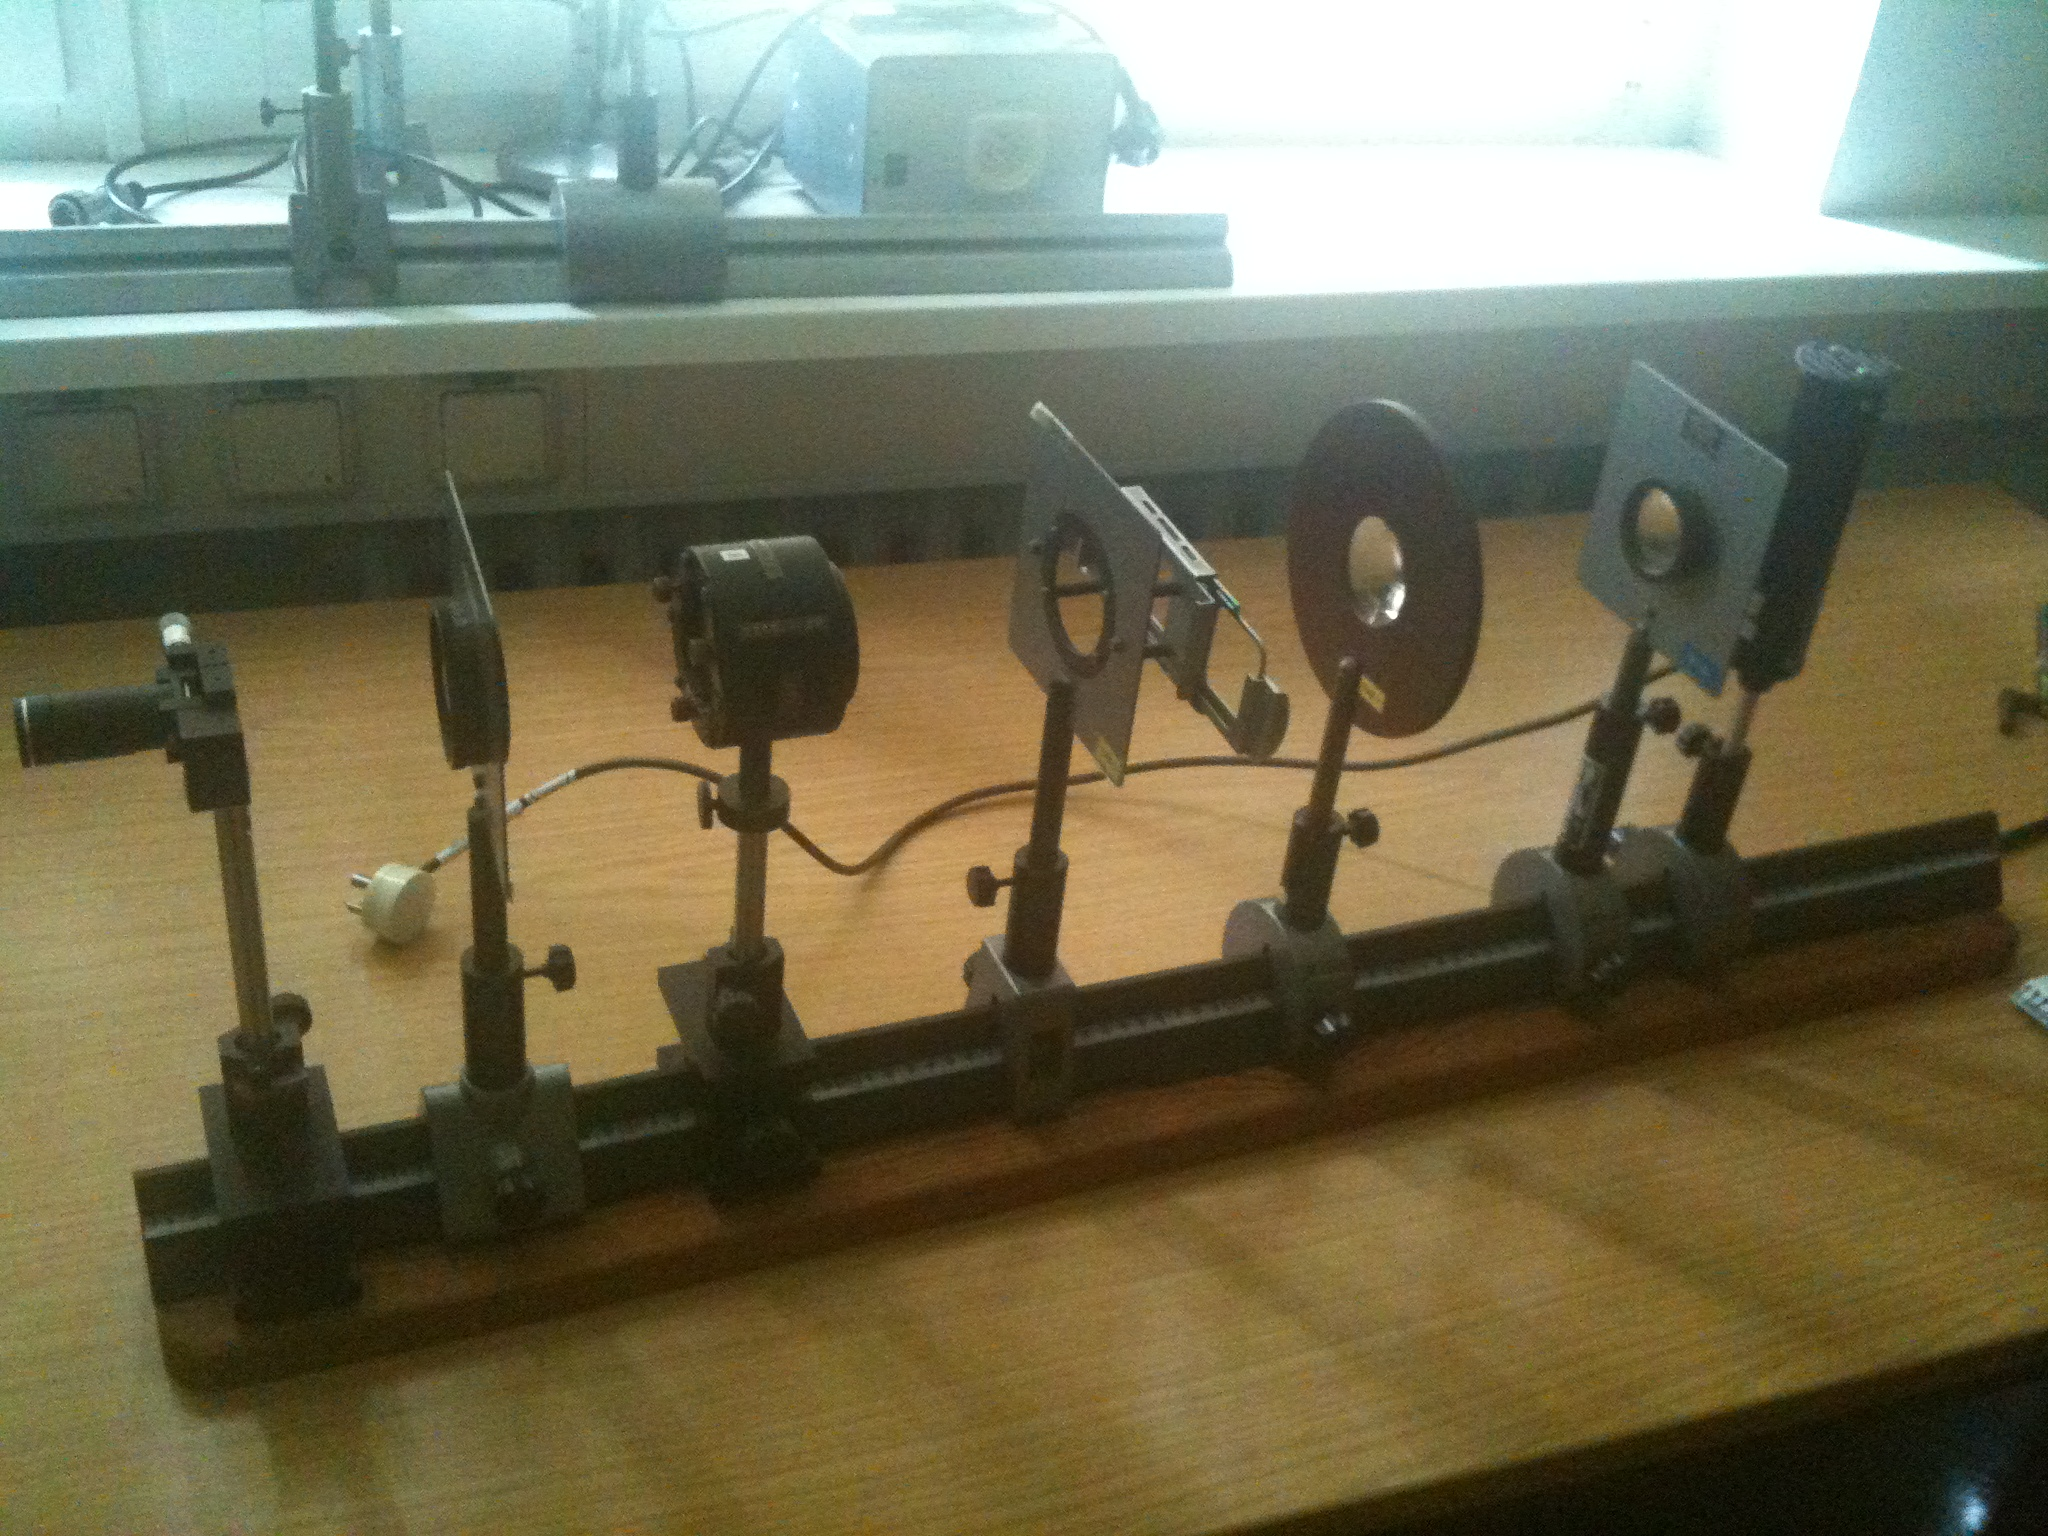
\includegraphics[width=8cm]{bilder/IMG_0021}}
\end{minipage}
\end{center}

Aufbau, von links nach rechts: 
\begin{itemize}
\item Okular
\item Objektivlinse $(f=100\pm 2)mm$
\item Etalon
\item Farbfilter
\item 1. Konvexlinse $(f=155\pm 2)mm$
\item 2. Konvexlinse $(f=120\pm 2)mm$
\item Cadmium-Lampe
\end{itemize}